  \documentclass[11,5 pt]{article}
\usepackage{natbib}
\usepackage{tikz,lipsum,lmodern}
\usepackage[most]{tcolorbox}
\usepackage{varwidth}
\usepackage{geometry}
\usepackage{url}
\usepackage[nottoc]{tocbibind}
\usepackage{fancyhdr}
\usepackage{enumerate}
\usepackage[utf8]{inputenc}
\usepackage{float}
\usepackage{caption}
\usepackage{subcaption}
\usepackage{cancel}
\usepackage{graphicx}               % Necessary to use \scalebox
\usepackage{textcomp}
\usepackage{amsmath}
\usepackage{dsfont}
\usepackage{cool}
\usepackage{enumitem}
\usepackage{csquotes}
\usepackage{comment}
\usepackage[sorting=none]{biblatex}
\bibliography{references}
\usepackage{tabularx}
\usepackage{chngcntr}
\usepackage[framed,numbered,autolinebreaks,useliterate]{mcode}
\usepackage{multicol}
\usepackage{enumitem,kantlipsum}
\usepackage[hidelinks]{hyperref}


\geometry{
 a4paper,
 total={160mm,223mm},
 left=25mm,
 top=42mm,
}

%% Definiciones de cuadros

\definecolor{anibalMorao}{HTML}{3366CC}

\newtcolorbox[auto counter,number within=section]{importanteBoxNumerado}[2][]{enhanced, colback=blue!5,colframe=blue!50,boxrule=0.4mm, attach boxed title to top left={xshift=1cm,yshift*=1mm-\tcboxedtitleheight}, varwidth boxed title*=-3cm, boxed title style={frame code={ \path[fill=tcbcolback!30!black] ([yshift=-1mm,xshift=-1mm]frame.north west) arc[start angle=0,end angle=180,radius=1mm] ([yshift=-1mm,xshift=1mm]frame.north east) arc[start angle=180,end angle=0,radius=1mm]; \path[left color=tcbcolback!60!black,right color=tcbcolback!60!black, middle color=tcbcolback!80!black] ([xshift=-2mm]frame.north west) -- ([xshift=2mm]frame.north east) [rounded corners=1mm]-- ([xshift=1mm,yshift=-1mm]frame.north east)
-- (frame.south east) -- (frame.south west)
-- ([xshift=-1mm,yshift=-1mm]frame.north west) [sharp corners]-- cycle; },interior engine=empty, }, fonttitle=\bfseries, title=Importante~\thetcbcounter. #2,#1}

\newtcolorbox[auto counter,number within=section]{destacadoBox}[2][]{enhanced,
colback=blue!5,colframe=blue!50,boxrule=0.4mm, attach boxed title to top left={xshift=1cm,yshift*=1mm-\tcboxedtitleheight}, varwidth boxed title*=-3cm, boxed title style={frame code={ \path[fill=tcbcolback!30!black] ([yshift=-1mm,xshift=-1mm]frame.north west) arc[start angle=0,end angle=180,radius=1mm] ([yshift=-1mm,xshift=1mm]frame.north east) arc[start angle=180,end angle=0,radius=1mm]; \path[left color=tcbcolback!60!black,right color=tcbcolback!60!black, middle color=tcbcolback!80!black] ([xshift=-2mm]frame.north west) -- ([xshift=2mm]frame.north east) [rounded corners=1mm]-- ([xshift=1mm,yshift=-1mm]frame.north east)
-- (frame.south east) -- (frame.south west)
-- ([xshift=-1mm,yshift=-1mm]frame.north west) [sharp corners]-- cycle; },interior engine=empty, }, fonttitle=\bfseries, title= #2,#1}

\newtcolorbox[auto counter,number within=section]{ejemploBoxNumerado}[2][]{enhanced,
colback=white,colframe=green!50,boxrule=0.4mm, attach boxed title to top left={xshift=1cm,yshift*=1mm-\tcboxedtitleheight}, varwidth boxed title*=-3cm, boxed title style={frame code={ \path[fill=tcbcolback!30!black] ([yshift=-1mm,xshift=-1mm]frame.north west) arc[start angle=0,end angle=180,radius=1mm] ([yshift=-1mm,xshift=1mm]frame.north east) arc[start angle=180,end angle=0,radius=1mm]; \path[left color=tcbcolback!60!black,right color=tcbcolback!60!black, middle color=tcbcolback!80!black] ([xshift=-2mm]frame.north west) -- ([xshift=2mm]frame.north east) [rounded corners=1mm]-- ([xshift=1mm,yshift=-1mm]frame.north east)
-- (frame.south east) -- (frame.south west)
-- ([xshift=-1mm,yshift=-1mm]frame.north west) [sharp corners]-- cycle; },interior engine=empty, }, fonttitle=\bfseries, title=Ejemplo~\thetcbcounter. #2,#1}

\newtcolorbox[auto counter,number within=section]{ejercicioBoxNumerado}[2][]{enhanced,
colback=red!5,colframe=red!50,boxrule=0.4mm, attach boxed title to top left={xshift=1cm,yshift*=1mm-\tcboxedtitleheight}, varwidth boxed title*=-3cm, boxed title style={frame code={ \path[fill=tcbcolback!30!black] ([yshift=-1mm,xshift=-1mm]frame.north west) arc[start angle=0,end angle=180,radius=1mm] ([yshift=-1mm,xshift=1mm]frame.north east) arc[start angle=180,end angle=0,radius=1mm]; \path[left color=tcbcolback!60!black,right color=tcbcolback!60!black, middle color=tcbcolback!80!black] ([xshift=-2mm]frame.north west) -- ([xshift=2mm]frame.north east) [rounded corners=1mm]-- ([xshift=1mm,yshift=-1mm]frame.north east)
-- (frame.south east) -- (frame.south west)
-- ([xshift=-1mm,yshift=-1mm]frame.north west) [sharp corners]-- cycle; },interior engine=empty, }, fonttitle=\bfseries, title=Ejercicio~\thetcbcounter. #2,#1}

\newtcolorbox[auto counter,number within=section]{notaNumerada}[2][]{colbacktitle=black!2!white, coltitle=red!70!black,fonttitle=\bfseries,title=Nota~\thetcbcounter. #2,#1,boxrule=0.1mm,colback=black!2}
\setlength{\parindent}{0pt}
\setlength{\parskip}{10pt}
\pagestyle{fancy}


\begin{document}
\begin{titlepage}

\centering

{\scshape\LARGE Navigating the Nexus: Climate Change, Clean Energy, and Nuclear Nonproliferation \par}
\begin{figure}[ht!]
\centering
\vspace{0.5 cm}

\includegraphics[scale=0.25]{images/gt-seal_0.png}
\end{figure}
\vspace{0.39 cm}

\centering

{\itshape\LARGE Review of existing literature within the NEXUS of Clean Energy, Nuclear Nonproliferation, and Climate Change to better understand the current status of the field.
 \par}
\vspace{1.3cm}
{\scshape\LARGE  FINAL UNDERGRADUATE RESEARCH REPORT\par}
\vspace{0.2 cm}

\vspace{1.5cm}
\begin{figure}[ht!]
\centering

\includegraphics[scale=0.08]{images/Initials.png}
\end{figure}
{\bfseries\LARGE Ethan Masters \par}
\vspace{0.55cm}
{\LARGE \textit{PI: Dr. Kosal \& Dr. Whitlark}\par}
\vspace{1.2cm}

{\Large May - August 2022 \par}
\end{titlepage}

\lhead{Final Undergraduate Research Report}
\rhead{ Ethan Masters }
\renewcommand{\headrulewidth}{0.5pt}

\tableofcontents

\newpage

\section{Introduction}
The global security implications of climate change are expected to result in unprecedented investments in alternative clean energy sources. Direct concerns of climate change include but are not limited to energy security, environmental migration, resource wars, and climate security \cite{scheffran2011climate}. Debates surrounding clean energy are multifaceted. It’s not the case that the most environmentally friendly energy source will be the main technology used in climate change mitigation strategies across the globe. Instead, factors like the current cost of such technologies and region-specific determinants will likely guide the mixed-use of clean energy technologies.

Energy decisions involve political, economic, and social aspects. Most plausible future scenarios of climate change mitigation include nuclear technologies in the zero-carbon energy mix. Nuclear power is currently the world’s second-largest source of zero-carbon baseload electricity, and its potential to improve energy security, spur economic growth, and reduce global emissions is significant. In 2021, the United States underscored this potential when Congress passed the bipartisan Infrastructure Investment and Jobs Act, allocating \$2.5 billion for R\&D in the next generation of advanced nuclear reactors. These small modular reactors (SMRs) are designed to lower construction costs and increase operational safety. The Department of Energy anticipates that demand for such advanced nuclear technologies could reach a trillion dollars in market opportunities – implying that the nuclear industry is poised to remain an indispensable component of the energy landscape. Notably, the nuclear industry’s influence extends beyond electricity generation; nuclear technologies find uses in medical treatments, industrial irradiation processes, and water desalination. In short, nuclear technology is likely here to stay despite the associated risks of nuclear weapons proliferation. This reality makes it all the more important for global security to understand and strategically manage how the increased use and advancement of nuclear technologies might produce adverse effects.

This literature review aims to survey existing research at the intersections of climate change, clean energy, and nuclear non-proliferation. The scholarship in this area is highly interdisciplinary. As noted above, there is relatively little work that explicitly examines all three facets together. This has necessitated breaking the problem into component pairs (dyads) and examining where two domains overlap as a foundation for understanding the triple nexus.


\subsection{Methodology}


Initial literature collection methods relied heavily upon Google Scholar and Scopus followed by reference tracing of relevant publications. Understanding the terminology of the academic field, coupled with the introduction of operators in the search query, helped refine output sources significantly. A temporal method was introduced to isolate publications in five-year intervals.

Other academic search engines including Scinapse, BASE, Semantic Scholar, The Lens, Scinapse, and Cambridge Core were also exhausted of relevant resources to the project’s scope. The types of literature collected included journal articles, review articles, books, world organization reports, and conference reports.

Literature citations were stored using EndNote, which offered advantages in sorting and reviewing publications. Citations were maintained with their respective PDF files in an online repository, which allowed for an isolated search query within the reference repository. This was especially useful while binning articles into sub-fields.
 

\subsection{Leximancer: Machine Learning Content Analysis Program}


\begin{figure}[H]
     \centering
         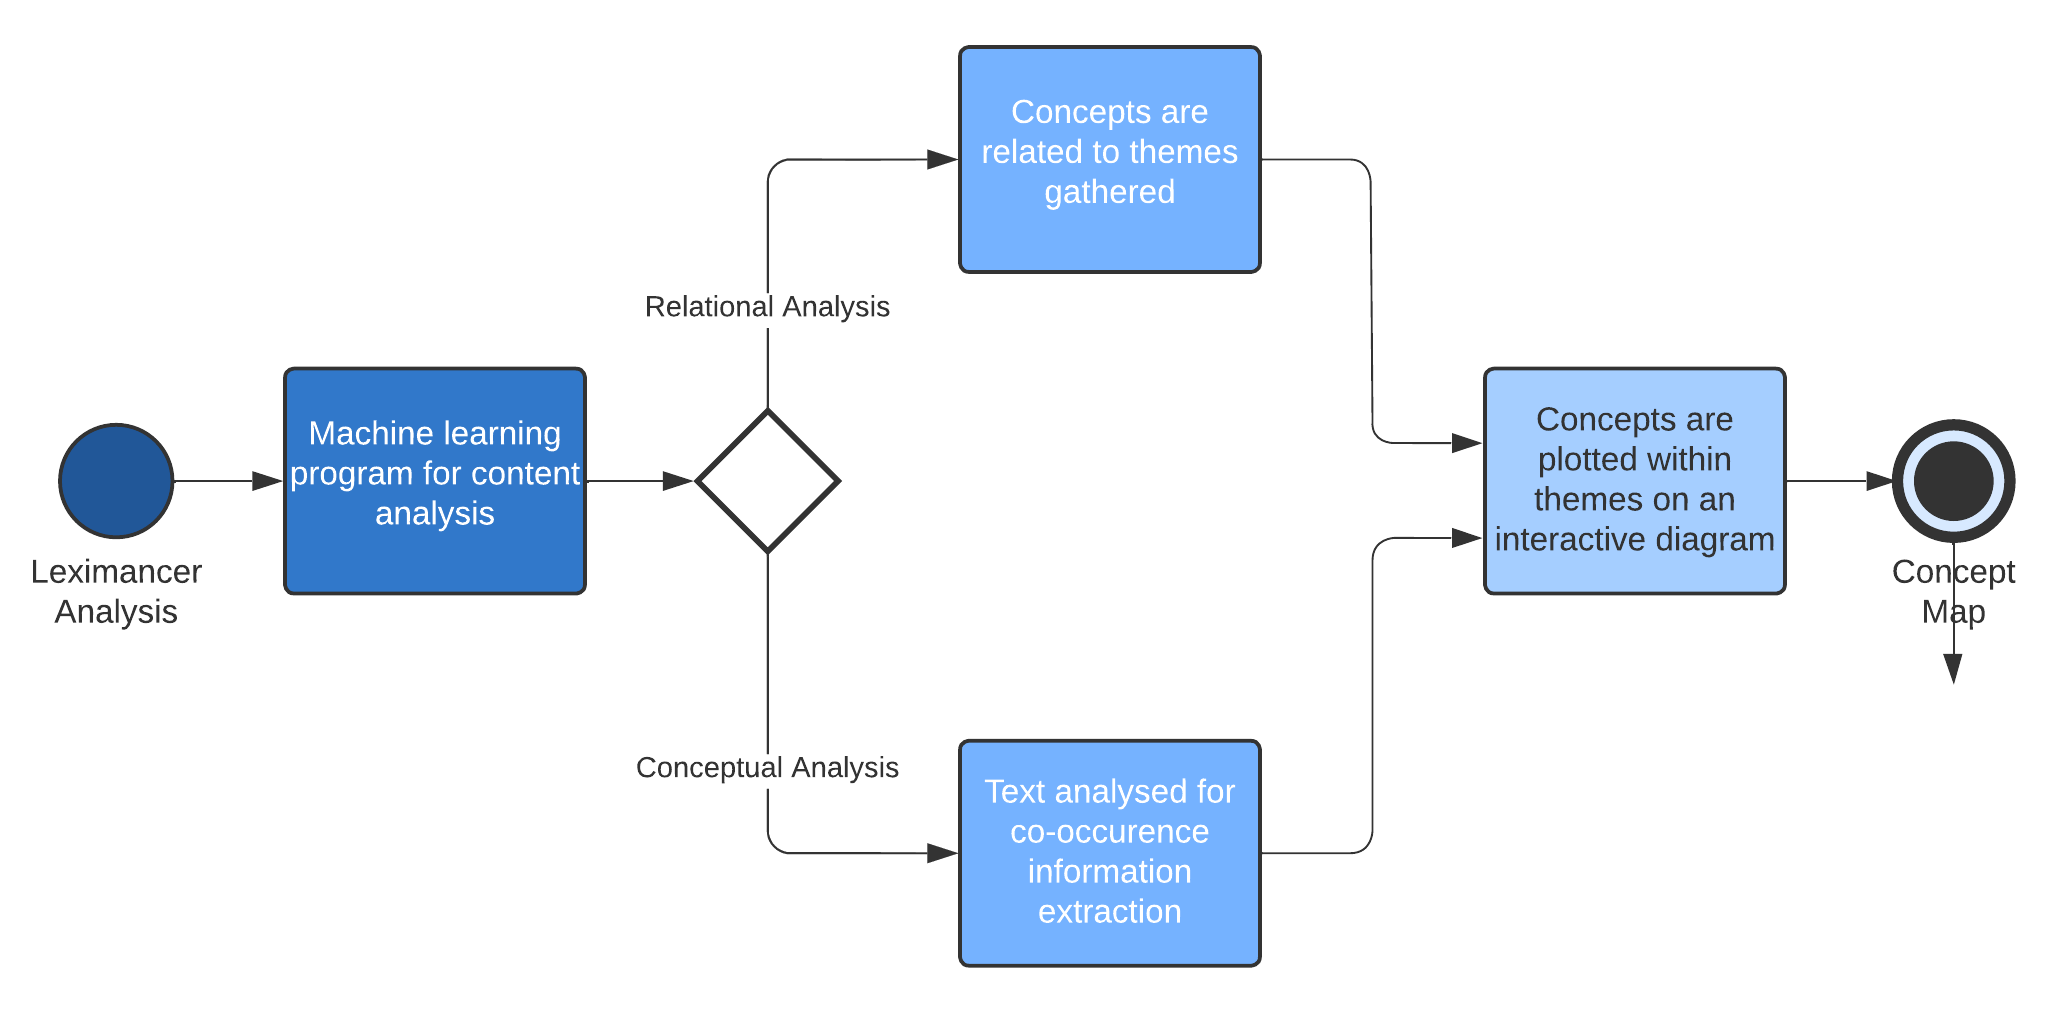
\includegraphics[scale=0.19]{images/BPMN 2.0 Example.png}
\caption{Leximancer Program Algorithm Flowchart \cite{Leximancer®}}
\label{Flowchart}
\end{figure}

Leximancer is a machine learning algorithm that produces a model for qualitative data analysis via two stages of co-occurrence information extraction: thematic and relational analyses. The program uses a method of transforming lexical co-occurrence information from natural language into semantic patterns. The algorithms are statistically based, but the program runs with nonlinear dynamics and utilizes machine learning \cite{Smith2006}. It has been cited in over 2000 journal articles and is considered one of the leading content analysis programs for research purposes. The tool automates text analysis by extracting high-level concepts from input documents and generates a concept map that visualizes these concepts and their relationships.

Leximancer not only develops the concept map shown in Figure 2, it also provides an alternative means to perform text analysis in an automated and systematic way using the semantic network developed by the program. The concept map can be thought of as a surface-level representation of the literature’s themes that can only be deeply interpreted using the underlying semantic network.


\subsubsection{Insights}


\begin{figure}[H]
     \centering
         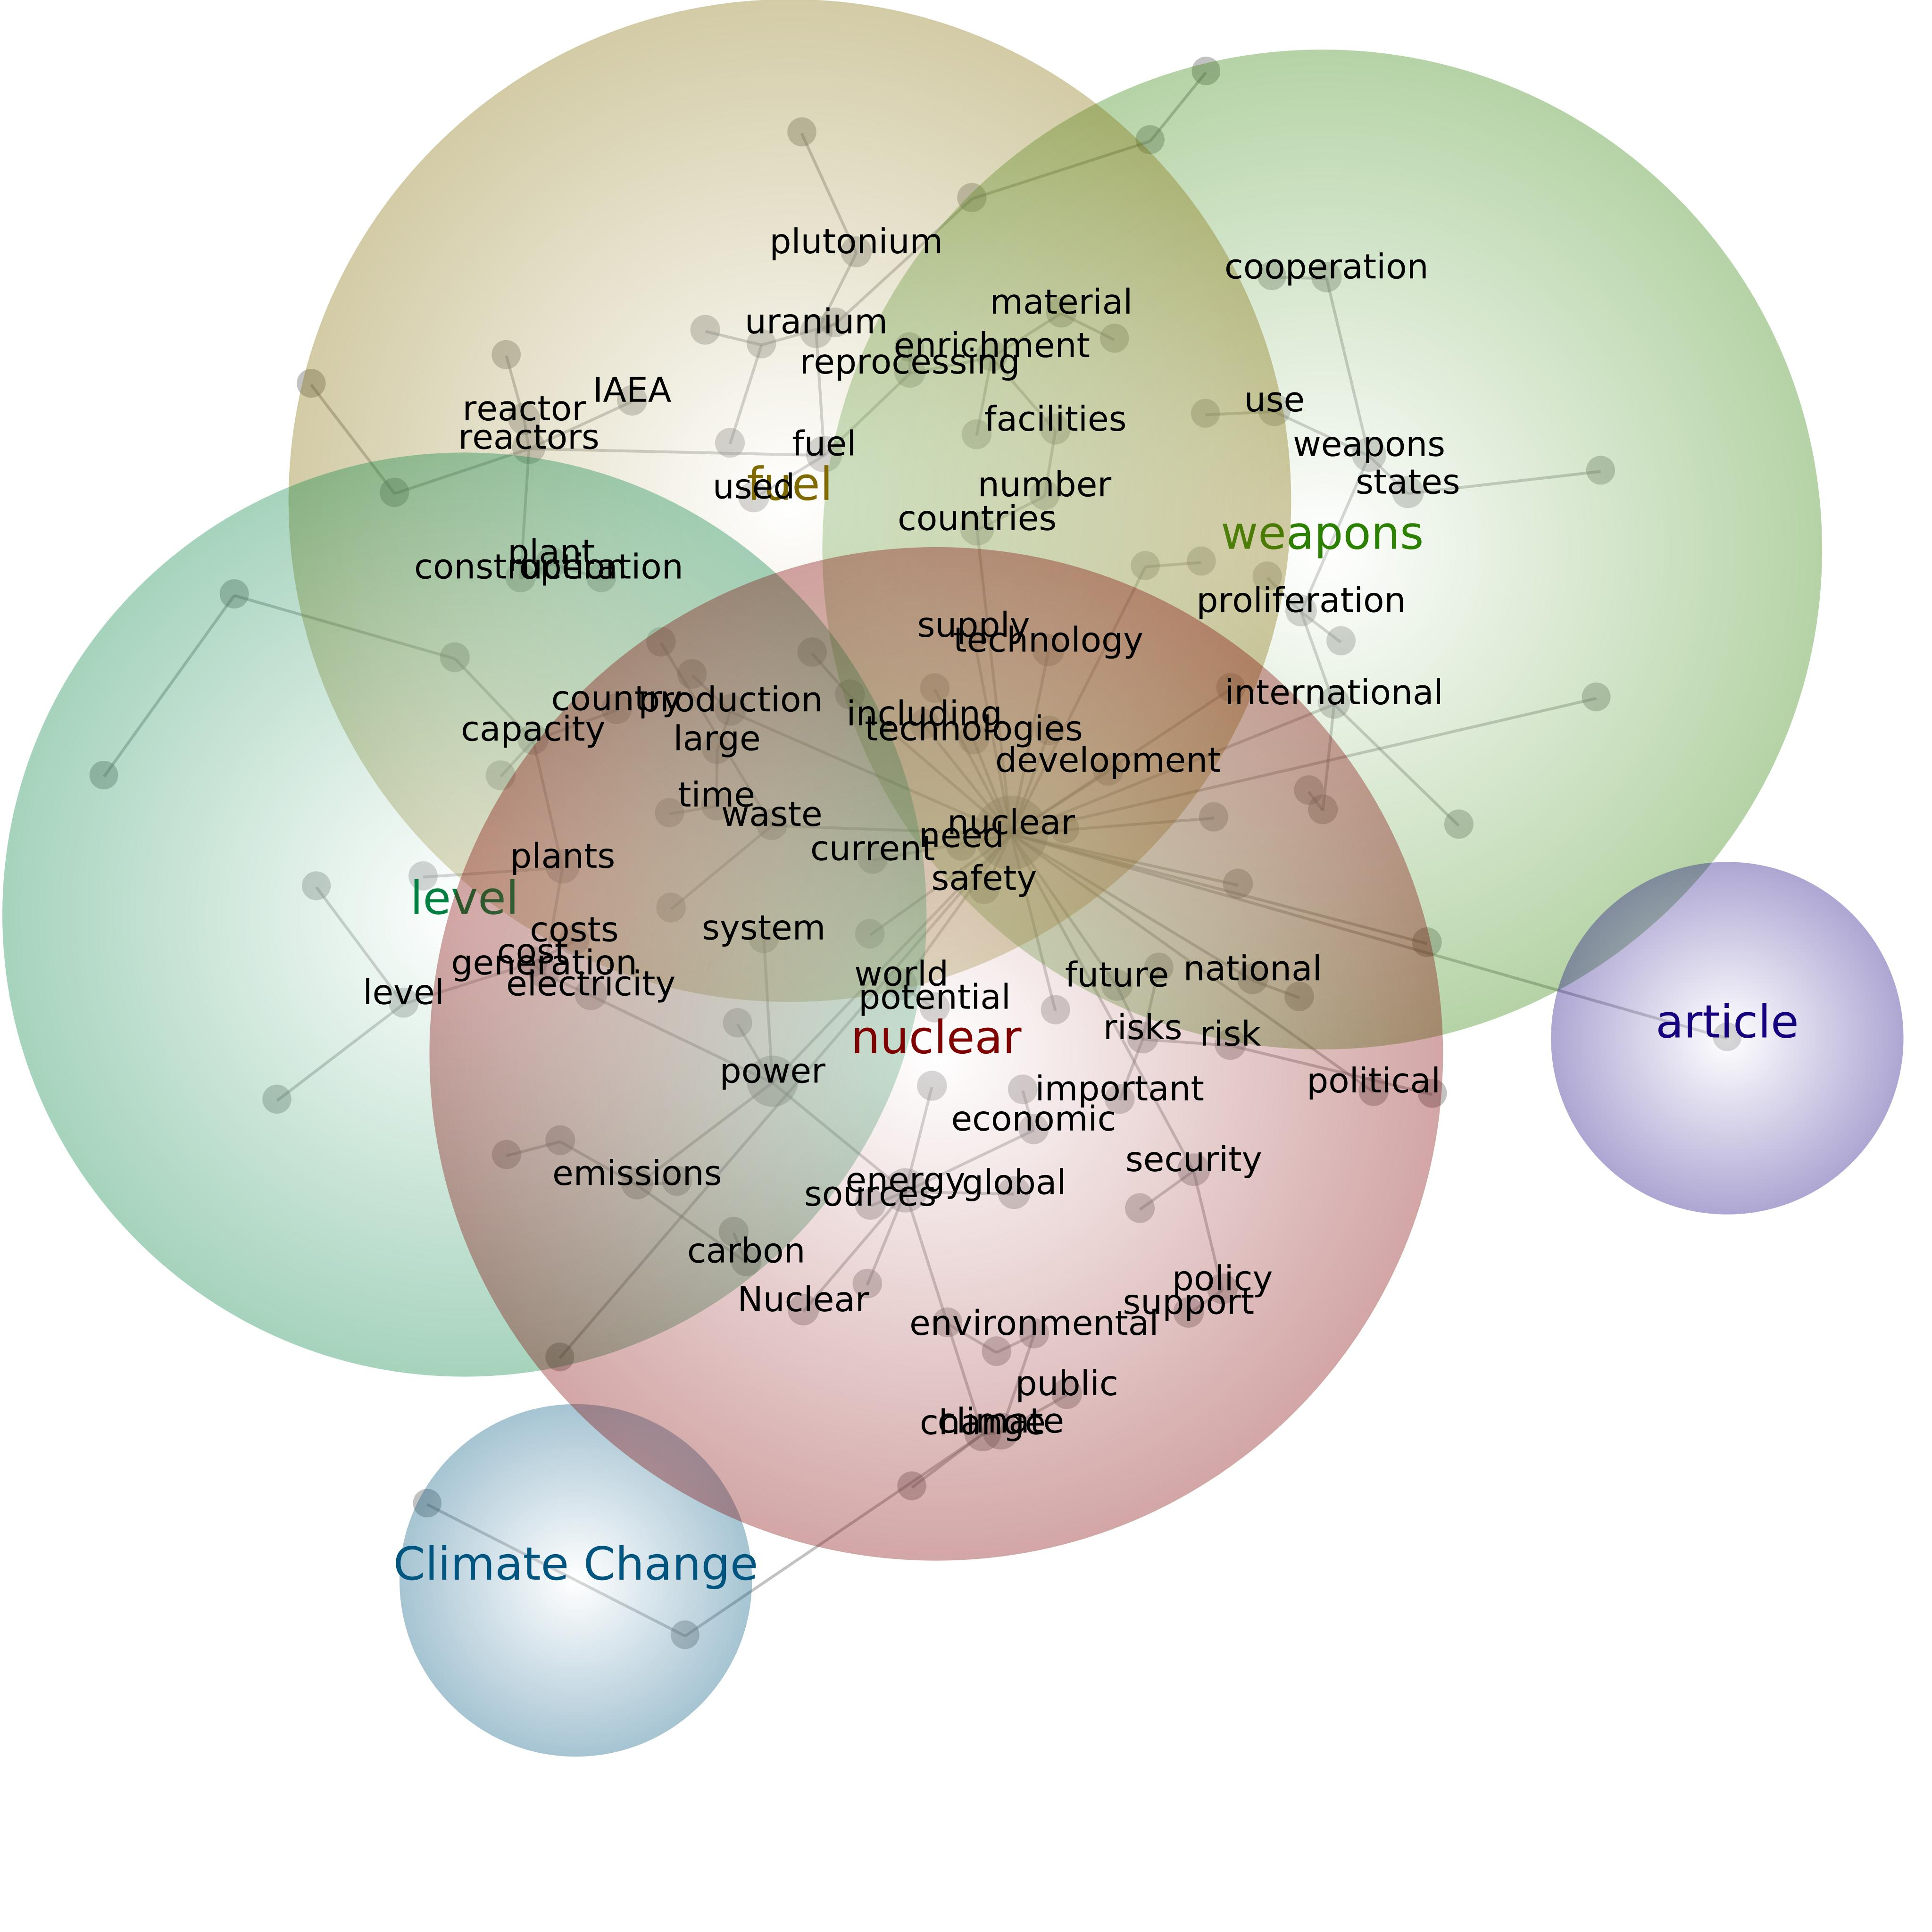
\includegraphics[scale=0.12]{images/E Nexus-concept-map.jpeg}
\caption{Qualitative Data Analysis Model of the NEXUS \cite{Leximancer®}}
\label{Qualitative}
\end{figure}


Initial insights were interpreted directly from the Leximancer concept map (Figure 2). The dominant theme in the map is \textit{nuclear}, which intersects with two other major themes: \textit{weapons} and \textit{energy}. It’s interesting to note that \textbf{Energy Policy} (a journal title) appears as a prominent term connecting the weapons and energy clusters, due to the copious amount of literature dealing with energy security, nuclear energy deployment, and the attendant risks of regional conflict or nuclear weapons proliferation. This underscores how central considerations of energy policy are to the study of clean energy and proliferation.

The size of the sub-themes in the concept map reflects their prominence in the literature. The main concepts identified include \textit{nuclear}, \textit{energy}, \textit{climate change}, \textit{global security}, \textit{weapons}, and \textit{safety}. This aligns with the focus of the collected literature: many works address the risks of nuclear technology proliferation and the impacts of climate change on the non-proliferation regime. Safety issues (such as the risk of nuclear accidents and the management of radioactive waste, which can harm the environment) also feature significantly.

By drilling deeper into the analysis, Leximancer also highlights several name-like concepts, with the most relevant being the \textbf{IAEA}, \textbf{United States}, \textbf{Russia}, and \textbf{China}. Leximancer’s ability to trace these names in context reveals how they figure in the literature. Indeed, many sources discuss the international nuclear technology market and emphasize the key role of Russia, as well as what the U.S. stands to lose if Russia continues to dominate that market. These insights from Leximancer reinforce the themes identified through manual review.

Leximancer also identified frequently used keywords (word-like concepts) such as \textit{nuclear}, \textit{power}, \textit{energy}, \textit{countries}, \textit{fuel}, \textit{reactors}, and \textit{technology}. The prominence of \textit{fuel} relates to discussions of the nuclear fuel cycle and the proliferation risks it entails. According to the concept map, \textit{fuel} is closely linked with \textit{IAEA}, \textit{Russia}, and \textit{United States}. This reflects the fact that the IAEA is responsible for regulating fuel reprocessing and enrichment to uphold NPT safeguards, and it will be pivotal in overseeing the security of expanding nuclear programs in the future. Russia’s presence in this context aligns with its known tendency to use energy exports as a tool of influence; similarly, Russia’s dominance in the nuclear fuel and reactor market poses concerns about new forms of energy dependency given its position as a leading supplier.


\section{Overview}


Climate change, clean energy, and nuclear nonproliferation form a complex nexus that has only recently begun to attract scholarly attention. Few comprehensive works explicitly address all three aspects together. In general, the literature tends to examine pairwise intersections—such as climate change and nuclear energy, or nuclear energy and proliferation—rather than the triple nexus. Nevertheless, several notable studies provide insight into how these domains intersect. For example, Sovacool (2012) analyzed the socio-political economy of nuclear power, discussing its role as a low-carbon energy source and its implications for global security governance \cite{Sovacool20121}. Weinberg et al. (1985) compiled perspectives on commercial nuclear power and proliferation, including how nuclear energy development affects climate mitigation prospects and nonproliferation efforts \cite{weinberg1985nuclear}. More recently, Scheffran \cite{scheffran2015climate} highlights potential linkages between climate change and nuclear risks, such as climate-induced conflicts that could heighten nuclear tensions and natural disasters threatening nuclear facilities. Bunn (2019) examined the requirements for large-scale nuclear energy deployment to meet climate goals, emphasizing the need for robust international verification and security measures to prevent the spread of nuclear weapons as nuclear power expands \cite{bunn2019nuclear}. These works underscore that nuclear energy often serves as the pivot linking climate change mitigation efforts with nuclear security concerns.

Because this integrated nexus is under-studied, research often focuses on the bilateral relationships within the trio. This review accordingly surveys literature in those overlapping areas as a basis for synthesis. Relevant studies appear across a range of disciplines, including climate policy, energy technology, and international security. Notably, a significant body of work is published in energy-focused journals such as \textit{Energy Policy}, which contributed many articles to this review. Other outlets, ranging from \textit{Progress in Nuclear Energy} to \textit{Daedalus} and security studies journals, have addressed pieces of the nexus – reflecting its interdisciplinary nature. In the following sections, we discuss key themes emerging at each of the major intersections: (1) nuclear energy as a clean energy option for climate change mitigation, (2) nuclear energy in the context of national and international security, (3) the implications of nuclear technology diffusion for the nonproliferation regime, and (4) public and political perceptions of the nuclear–climate interface. Throughout, we highlight points of consensus and disagreement in the literature and identify where the three topics converge.


\section{Nuclear Energy at the intersection of Climate Change Mitigation \& Clean Energy Technologies}


A central question in the nexus is whether nuclear energy can serve as a viable clean energy solution for climate change mitigation. Many studies contend that nuclear power will indeed form part of the portfolio of low-carbon technologies needed to achieve global emissions reduction targets. Nuclear power already provides a substantial share of carbon-free electricity worldwide and has historically averted billions of tons of greenhouse gas emissions. Unlike intermittent renewables, it offers steady baseload generation, and it may also facilitate deep decarbonization in other sectors (for instance, by producing hydrogen fuel through nuclear-powered electrolysis). Some analyses argue that without an expansion of nuclear power, the world’s growing energy demand cannot be met while keeping greenhouse gas levels in check. For example, Duffey (2005) emphasizes the “particularly important role” for nuclear power in enabling a sustainable, low-carbon future, highlighting its potential to support a hydrogen economy and complement renewable sources \cite{DUFFEY2005535}. In line with this, energy-economy models and scenario studies – including those informing international climate policy – often include nuclear alongside renewables and efficiency measures as part of the cost-effective mitigation mix needed to reach net-zero emissions.

However, there is considerable debate about the extent to which nuclear energy can and should contribute to climate goals. A number of scholars point to economic and temporal constraints that may limit nuclear power’s role. Nuclear plants are capital-intensive and have long development timelines, with historical trends of cost escalation and project delays – challenges that were evident even before the added safety requirements imposed after accidents like Fukushima. As Kessides (2012) observes, more stringent regulations following the 2011 disaster have further increased nuclear costs and undermined its economic viability, unless next-generation designs can significantly reduce these hazards and costs \cite{KESSIDES2012185}. Indeed, the promise of advanced reactors such as SMRs is frequently cited as a way to address some of these issues: by downsizing reactors to simpler, standardized units, SMRs aim to lower construction costs and financial risk, potentially making nuclear projects more manageable. Whether such innovations can deliver in time to meaningfully aid climate mitigation remains uncertain. Meanwhile, some empirical studies question nuclear energy’s effectiveness in practice as a climate solution. Gralla et al. (2017) found no clear evidence that national adoption of nuclear power correlates with lower carbon emissions or improved energy access outcomes, casting doubt on the idea that nuclear is a universal answer to global challenges like climate change \cite{GRALLA20171251}. Similarly, Marignac (2015) argues that the nuclear option entails intrinsic risks – including weapons proliferation, reactor accidents, and long-lived waste – and notes that even a maximal nuclear build-out would have only a limited impact on reducing greenhouse emissions relative to its scale. Critics also contend that every dollar spent on expensive nuclear projects might achieve greater and faster emissions cuts if invested in renewable energy or efficiency, given the rapidly falling costs of those alternatives (a point made forcefully by Lovins \cite{LOVINS2022107122} in the U.S. context). Thus, the literature reveals a distinct divide: some analysts portray nuclear power as an indispensable tool for deep decarbonization and energy security, while others view it as an economically strained and slow-to-deploy option that could divert resources from more effective climate actions.

This divergence in views underscores that the role of nuclear energy in a clean energy transition will likely depend on policy choices and public acceptance as much as on technical merits. Implementing climate strategies that include nuclear power requires addressing its challenges through supportive policies (such as carbon pricing or subsidies for advanced reactor deployment) and robust safety and waste management frameworks. Importantly, any substantial expansion of nuclear generation for climate purposes also raises questions about nuclear weapons proliferation and security, due to the dual-use nature of nuclear technology. As discussed in the next sections, the prospect of dozens of new nuclear reactors worldwide – especially in regions new to nuclear energy – has prompted extensive analysis of how to prevent the spread of nuclear weapons capabilities under the guise of civilian programs. In short, the clean energy benefits of nuclear power cannot be separated from these broader security considerations.


\section{Nuclear Energy at the Intersection of Climate Change and National Security}


Expanding nuclear energy to combat climate change has ramifications beyond the environmental sphere; it is also tightly interwoven with issues of national and international security. One reason is that energy is a strategic domain: countries often view civilian nuclear power programs through the lens of energy security and geopolitical influence. On the one hand, adopting nuclear energy can reduce a state's dependence on imported fossil fuels, theoretically enhancing energy independence and resilience in the face of climate change policies that constrain carbon emissions. On the other hand, because nuclear technology and fuel supply are concentrated in the hands of a few supplier nations, new nuclear energy users may simply trade one form of dependency for another. In practice, most countries embarking on nuclear power rely on foreign vendors for reactor technology, fuel, and operational support. This creates long-term interdependencies: for example, Russia, France, the United States, China, and a handful of others collectively account for over 90\% of global nuclear export agreements. Notably, Russia alone has been the supplier in roughly half of all international nuclear reactor deals in recent decades, giving it enormous leverage. Such leverage is not merely hypothetical: Russia has a documented history of using energy exports as a foreign policy tool, and observers warn that it could similarly “weaponize” its dominant position in the nuclear energy market to exploit client states’ dependencies. Moscow’s Build-Own-Operate (BOO) model for reactor projects, whereby Russia provides financing, construction, and fuel while retaining ownership and operation of the plant, effectively locks recipient countries into reliance on Russian services for decades. China has pursued a comparable strategy by exporting reactors under its Belt and Road Initiative, an effort that not only seeks new markets but also extends Chinese geopolitical influence and potentially shapes new norms around nuclear governance. These developments raise concerns that the decarbonization of the global energy system—if achieved in part via a worldwide “nuclear renaissance”—could introduce new patterns of great-power influence and rivalry, with Russia and China in particular capitalizing on their role as nuclear technology suppliers. Western analysts note that this trend could undermine international security: if authoritarian supplier states set the terms of nuclear expansion, safety and nonproliferation standards may be weakened. Consequently, several experts argue that it is in the interest of the United States and its allies to remain actively engaged in the global nuclear energy arena. Gattie (2020), for instance, contends that the U.S. civilian nuclear industry should be treated as a strategic national asset, warning that if America retreats while “competing powers are leveraging civilian nuclear collaboration to meet strategic geopolitical objectives,” those rival powers will become the world’s nuclear leaders “with adverse implications for U.S. national security” \cite{10.2307/26937414}. In line with this, policy proposals urge the U.S. to bolster international nuclear cooperation initiatives and help strengthen global norms (such as nonproliferation rules and safety standards) so that the clean energy transition does not come at the cost of a more precarious security environment \cite{LOVERING2020111306}.

Another security dimension of the climate–nuclear nexus arises from the potential link between civilian nuclear programs and nuclear weapons proliferation. The technologies used for nuclear energy (notably uranium enrichment and spent fuel reprocessing) can be dual-use, meaning that ostensibly peaceful programs might also enable a country to acquire weapons-usable nuclear material. Thus, when states announce nuclear power ambitions—often justified by legitimate energy or climate goals—neighbors and rivals may become suspicious of hidden military intent. Historical cases underscore this point: Pradhan (2010) documents how plans for nuclear power in West Asian countries like Saudi Arabia were perceived as strategic moves to counter regional adversaries (in Saudi’s case, Iran’s nuclear program), raising fears of a Middle Eastern nuclear arms race under the guise of civil energy needs \cite{Pradhan2010843}. More generally, the expansion of nuclear energy in regions of geopolitical tension could exacerbate security dilemmas, as states worry that their opponents’ reactors might one day yield plutonium for bombs or that nuclear infrastructure could be targeted in conflicts. Climate change adds further complexity to this picture. Some analysts posit that as climate impacts (such as water scarcity or natural disasters) stress state stability, the risk of conflict increases – and any such conflicts involving nuclear-armed states or nuclear facilities carry heightened stakes. Scheffran et al. (2015) argue that climate-induced crises could indirectly elevate nuclear risks — for example, a climate-driven resource war could trigger nuclear brinkmanship, or extreme weather events could threaten the safety of nuclear plants, compounding disaster scenarios \cite{scheffran2015climate}. While these worst-case linkages remain speculative, they illustrate how climate security and nuclear security considerations are becoming increasingly intertwined.

In summary, the pursuit of nuclear energy as part of a clean energy transition is not occurring in a geopolitical vacuum. It has the potential to reshape international alignments and affect national security calculations. Ensuring that this transition strengthens rather than undermines global security will require proactive governance – from preventing exploitative reactor deals and maintaining rigorous safety norms, to building confidence that civil nuclear cooperation will not spiral into regional arms races. These challenges directly connect to the nonproliferation regime, which we examine in the next section.


\section{Nuclear Technologies \& the Nuclear Non-Proliferation Regime}


The prospect of a global nuclear energy expansion has intensified focus on the nuclear non-proliferation regime and its ability to prevent the misuse of nuclear technology. Civilian nuclear power programs operate under international agreements (primarily the Nuclear Non-Proliferation Treaty, or NPT) that seek to ensure countries can access nuclear energy for peaceful purposes without acquiring nuclear weapons. This balance becomes more precarious as more nations adopt nuclear technology or as existing nuclear states scale up their programs in response to climate change. A core concern is that the same technologies enabling nuclear power—especially uranium enrichment and plutonium reprocessing—can be reconfigured to produce the fissile material for nuclear warheads. Lehtveer (2014) observes that if nuclear power is to make a significant contribution to climate mitigation, it would necessitate the global diffusion of enrichment and reprocessing capabilities (or alternative fuel cycles), which in turn would heighten proliferation risks unless new safeguards are in place \cite{doi:10.1080/13669877.2014.889194}. Goldston (2011) similarly notes that the magnitude of nuclear deployment required for deep decarbonization would vastly increase the circulation of weapons-usable materials, demanding correspondingly stronger measures to prevent their diversion to military use \cite{Goldston}. In essence, an era of expanded nuclear energy could put unprecedented strain on the existing nonproliferation regime, which was not originally designed to monitor and secure nuclear activities on the scale now being contemplated.

To address these challenges, scholars and policymakers have proposed a range of strategies to adapt or strengthen the nonproliferation regime in parallel with any nuclear energy renaissance. A recurring theme is the internationalization of the nuclear fuel cycle. Rather than each country developing sensitive fuel-cycle facilities, multinational approaches have been advocated to keep enrichment and reprocessing under tighter international control. Feiveson (2008), Socolow (2009), and others argue that future large-scale nuclear power must be accompanied by multinational or international ownership of enrichment and reprocessing plants, along with a halt to the separation of plutonium, in order to “decouple nuclear power from nuclear weapons” \cite{10.2307/resrep05034} \cite{10.2307/40543999}. In line with this thinking, Goldschmidt (2010) outlines how multilateral fuel supply centers and spent fuel repositories could ensure reliable access to nuclear fuel services for all participants while removing incentives for states to build indigenous enrichment or reprocessing facilities \cite{goldschmidt2010multilateral}. The idea of an international fuel bank, backed by the IAEA and other agencies, has been put forward as a practical mechanism to assure reactor fuel supply and thereby dissuade national fuel-cycle ventures. Saltiel (2005) likewise stresses the importance of establishing a multinational enrichment program to mitigate proliferation dangers \cite{saltiel2005strengthening}, and modeling studies by Crozat et al. (2004) suggest that arrangements like global nuclear fuel leasing—wherein a supplier provides fresh fuel and takes back spent fuel—could significantly reduce proliferation risks if coupled with rigorous safeguards \cite{SpentFuelModel}. At the same time, analysts acknowledge substantial obstacles to these solutions: Álvarez-Verdugo (2010) identifies economic, political, and legal hurdles that would need to be overcome to implement a truly multilateral enrichment and recycling system, such as reconciling national sovereignty over nuclear technology with international control, and aligning the interests of both established nuclear states and newcomers \cite{Milagros}.

Another avenue for reducing proliferation risk is technological innovation aimed at “proliferation-resistant” nuclear energy systems. For instance, certain Generation IV reactor designs and advanced fuel cycles are being developed with the goal of producing less weapons-usable material or even consuming existing stockpiles of plutonium, thereby supporting nonproliferation and disarmament efforts simultaneously. While no technology can be entirely proliferation-proof, the integration of intrinsic barriers (like fuels that are difficult to weaponize) and enhanced safeguardability in new reactor designs could complement institutional measures. Likewise, strengthening international safeguards and security practices is essential. Williams and Feiveson (1990) argued for developing clear “diversion-resistance” criteria for future nuclear systems, warning that current safeguards would be inadequate if nuclear power expanded dramatically without major reforms \cite{williams1990diversion}. Today, this implies bolstering the IAEA’s resources and authority for inspections, adopting real-time monitoring technologies, and improving material accountancy to cope with larger quantities of nuclear material spread across more sites.

Despite these proactive measures, some researchers remain skeptical about our ability to fully eliminate proliferation risks amid a nuclear resurgence. Historical studies of nuclear technology transfer suggest that even civilian cooperation can contribute to weapons proliferation over time. Bluth (2010), for example, provides evidence that states receiving peaceful nuclear assistance have been more likely eventually to initiate nuclear weapons programs, creating a causal link between civilian nuclear cooperation and proliferation outcomes \cite{10.2307/40784651}. This finding serves as a caution that well-intentioned nuclear aid (for energy or climate reasons) might inadvertently facilitate the spread of nuclear weapons capabilities. It underscores the importance of stringent export controls (such as those coordinated by the NSG) and the need for transparency and confidence-building measures when countries embark on nuclear energy programs.

Finally, many experts underline that the success of nonproliferation in a world with more nuclear energy will depend on broader political conditions, including progress in nuclear disarmament. If nuclear-armed states reduce their arsenals and strengthen their own compliance with nonproliferation norms, it could create a more conducive environment for expanded peaceful use of nuclear technology. Some have argued that visible disarmament steps would help persuade non-nuclear-weapon states that an expansion of nuclear power will not lead to a new wave of weaponization. Conversely, if nuclear weapons remain central to national security doctrines, the spread of nuclear power to new states will continue to carry a latent weapons risk. In short, reconciling a nuclear energy expansion with nonproliferation requires a holistic approach: technical safeguards, international institutional innovation, and a supportive geopolitical climate all play a role.


\section{Transnational Nuclear Technology Market and Non-proliferation}


A recurrent concern in the literature is whether the global nuclear technology market is evolving in a way that strengthens or undermines non-proliferation efforts. As demand for nuclear energy potentially grows under climate change policies, the structure and governance of the nuclear export market take on heightened importance. The international nuclear marketplace is relatively concentrated: for decades, a small number of nations (and their corporations) have dominated the supply of reactors, fuel, and related services. Traditionally, this market was led by Western suppliers under frameworks like the Nuclear Suppliers Group (NSG), which coordinate export controls and ensure recipients meet non-proliferation criteria. However, the landscape is shifting. The rise of state-backed suppliers from Russia and China, and the ambitions of new entrants, are creating a more complex and in some ways less transparent network of nuclear commerce. Nguyen (2019) notes that the nuclear export market has become “more concentrated and uncertain,” with emerging suppliers not fully participating in the established non-proliferation regime and newcomer customer states often possessing weaker governance capabilities \cite{Nguyen}. In other words, some of the countries now actively promoting or receiving nuclear technology may not be as embedded in the web of agreements and best practices that historically mitigated proliferation risks.

One implication is that nuclear deals may increasingly occur outside the strict oversight of traditional non-proliferation institutions. For example, if a newcomer nuclear state purchases a reactor from a supplier that is less stringent about safeguards or transparency, the risk of inadequate security or covert misuse could rise. The literature points out that the IAEA, while central to verifying compliance through safeguards, has limited authority over bilateral nuclear commerce and cannot fully police the transfer of technology on its own. This gap is especially concerning in light of geopolitical trends: as discussed earlier, Russia’s and China’s growing role in exporting reactors could potentially dilute the influence of Western conditionalities (such as requiring robust safeguards or adherence to treaties) in nuclear agreements. Some analyses, like Yusof (1986), have examined how supplier states balance commercial interests with non-proliferation commitments. The challenge today is that not all nuclear suppliers share the same non-proliferation norms or transparency standards; competition for reactor contracts might drive some providers to offer more lenient terms, undercutting the strict standards set by others.

Furthermore, a larger and more dispersed global nuclear industry heightens concerns about nuclear security — the protection of nuclear materials and facilities against theft, sabotage, or terrorism. The risk is not only state-level proliferation but also the possibility that terrorist organizations could exploit weaker links in the global system. As more nuclear material is produced and transported internationally, ensuring its security becomes paramount. Researchers like Bevins (2017) have explored the plausibility of non-state actors acquiring special nuclear material from civilian stocks, concluding that while it is difficult, it is not impossible without stringent preventative measures \cite{bevins2017alternate}. Past incidents of illicit nuclear technology trafficking (such as the A.Q. Khan network) illustrate how gaps in international oversight can be exploited, leading to proliferation in unexpected ways. Recognizing this, experts call for strengthening the global nuclear security architecture in parallel with any expansion of nuclear energy. This includes bolstering initiatives for real-time tracking of nuclear materials, peer-review mechanisms for national security practices, and expanding training and resources to countries new to nuclear energy so they can uphold high security standards. International cooperation is also emphasized: for instance, Lovering et al. (2020) outline strategies the United States might adopt or promote — such as international fuel leasing, tighter security exercises, and offering attractive alternatives to at-risk nations — to ensure that as the market evolves, it does so in a way that maintains robust non-proliferation and security norms.

In summary, the globalization of nuclear energy presents a double-edged sword. On one side, sharing nuclear technology can help meet global energy and climate goals; on the other, it introduces proliferation and security risks that transcend national borders. The transnational nature of the nuclear industry means that weaknesses in one country’s regulations or practices can reverberate globally. The literature highlights the need for updated international frameworks — perhaps expanding the mandate of the IAEA or revitalizing NSG guidelines — to keep pace with the changing market. It also underscores the importance of major powers working in concert to set high standards for nuclear exports, so that the clean energy benefits of nuclear technology do not come at the expense of weakened controls on some of the world’s most dangerous materials.


\section{Nuclear Renaissance \& Risks of Proliferation}


The term “nuclear renaissance” was used to describe a predicted revival of nuclear power worldwide in the early 21st century, driven by rising energy needs and climate change mitigation goals. Although the expansion of nuclear energy since 2000 has been slower than anticipated – dampened by high costs and events like the Fukushima accident – many countries continue to explore nuclear power options, and climate imperatives could renew momentum for nuclear development. The prospect of dozens of new reactors and new nuclear nations in the coming decades has generated a substantial body of literature concerned with making such a renaissance compatible with non-proliferation. Much of this literature reiterates and expands upon the themes discussed above. For example, Feiveson (2008) and Socolow (2009) argue that without fundamental changes such as multinational control of fuel-cycle facilities and a cessation of national plutonium separation, a worldwide expansion of nuclear power will carry unacceptable proliferation risks \cite{10.2307/resrep05034} \cite{10.2307/40543999}. Goldschmidt (2010) likewise advocates for internationally managed fuel supply and waste management as priorities to support any growth in nuclear energy while keeping the spread of sensitive technologies in check. These scholars tend to conclude that a robust international regime – more intrusive and cooperative than today’s – could, in principle, allow a major increase in nuclear energy use without a commensurate increase in nuclear weapons proliferation.

Other research is more skeptical, emphasizing uncertainties and the historical record of proliferation. Kim (2022) analyzes contemporary shifts in civil nuclear cooperation, such as the emergence of new supplier-recipient partnerships outside the traditional West-to-rest paradigm, and concludes that evolving power dynamics could introduce additional proliferation uncertainty \cite{KIM2022112852}. Bluth (2010), as noted earlier, finds an empirical link between civilian nuclear assistance and weapons proliferation, casting doubt on the notion that a dramatic expansion of nuclear energy can be completely insulated from the spread of nuclear arms. Bunn (2019) and other policy analysts stress the need for unprecedented levels of transparency, verification, and international cooperation if we are to manage the dual risks of climate change and proliferation simultaneously. Some voices, such as Benea (2011), even suggest that significant global nuclear growth should be deferred until further progress is made on nuclear disarmament – on the logic that as long as nuclear weapons retain their prestige and value in international politics, an expansion of nuclear energy will always carry a latent risk of weapons ambitions \cite{benea2011atom}. 

In essence, the debate around a nuclear renaissance encapsulates a broader tension: can the world significantly increase its reliance on nuclear power – a technology inherently capable of destruction as well as creation – without undermining international security? The optimistic view is that through rigorous multilateral governance and technological safeguards, the benefits of nuclear energy for climate mitigation can be realized with minimal proliferation risk. The pessimistic view counters that human and institutional fallibilities, and the realities of international rivalry, make it likely that more nuclear activity will sooner or later lead to more nuclear weapons capabilities. This unresolved debate highlights the importance of continued innovation in policy and technology, as well as close monitoring of how the next chapter of nuclear energy development unfolds.


\section{Attitudinal Nexus of Nuclear \& Climate Change}


Public perception and acceptance emerge as pivotal factors at the nexus of nuclear energy and climate change. In recent years, as governments pursue decarbonization, there have been concerted efforts to reframe nuclear power in the public discourse as not just an energy source, but also a climate change solution. The United Kingdom offers an illustrative case: after years of public skepticism toward nuclear power, the mid-2000s saw a policy reversal wherein nuclear energy was explicitly promoted as a “green” option to combat climate change. Doyle (2011) documents how the UK news media contributed to this reframing, increasingly portraying nuclear power as a low-carbon answer to global warming and signaling a dramatic shift from the government’s prior commitment to phase out existing nuclear plants \cite{Doyle}. Similarly, Bickerstaff et al. (2008) show that climate change and energy security narratives have been used to shift the debate around nuclear power in the UK, presenting it as part of the solution to urgent low-carbon energy needs – although concerns about radioactive waste remain a persistent counterpoint in public discourse \cite{Bickerstaff}. These reframing strategies indicate that the climate crisis is being leveraged to improve public attitudes toward nuclear energy.

Whether such strategies succeed, however, depends on public values and context. Research on public opinion reveals nuanced and sometimes ambivalent views. In Britain, Corner et al. (2011) found that concern about climate change and energy security can lead to greater openness to nuclear power, but only under specific conditions – essentially, the public’s acceptance increased “conditionally,” once other preferred options like renewable energy and conservation were perceived as insufficient \cite{CORNER20114823}. In other words, many people might accept nuclear energy if they become convinced that alternatives alone cannot meet the country’s needs, but if those alternatives seem viable, nuclear remains a less desirable choice. A broader European study by Pampel (2011) likewise found relatively low overall support for nuclear energy even among citizens highly concerned about climate change \cite{Pampel}. Instead, factors such as socio-economic status and familiarity with nuclear technology were more strongly associated with pro-nuclear views: at the individual level, higher socioeconomic status tended to increase support for nuclear energy, and at the national level, the presence of operating nuclear power plants correlated with higher public support. This suggests that abstract appreciation of nuclear’s climate benefits is often not enough to win over skeptics; personal and national context – including trust in institutions and direct experience with nuclear energy – strongly shape attitudes.

Public opinion in other parts of the world reflects similar complexity. In China, where the government actively promotes nuclear power for energy and climate objectives, a survey by Wang et al. (2013) indicated that attitudes toward nuclear power were complex and sometimes uncertain \cite{wang2013impact}. Notably, the study suggested that framing nuclear development as a response to climate change or to pressing energy security needs could increase public support, but that support was conditional and not without reservations. One key determinant of public acceptance is trust. Vainio et al. (2017) examined how trust in different information sources correlates with perceptions of the risks of nuclear energy versus the risks of climate change \cite{Vainio2017WeighingTR}. They found that individuals who trust scientific and governmental information sources are more likely to view nuclear power’s risks as acceptable given the threat of climate change, whereas those who are distrustful of authorities tend to remain opposed to nuclear even in the face of climate concerns. This indicates that public acceptance is not driven solely by facts about carbon emissions, but also by confidence in how nuclear risks are managed and communicated.

Another intriguing aspect of public attitudes is the psychological linkage between nuclear weapons and nuclear energy. For many people, these two facets of “the nuclear” are intertwined in perception. Baron et al. (2020) investigated this attitudinal nexus in the United States and found evidence that opposition to nuclear weapons often goes hand-in-hand with opposition to nuclear energy \cite{BARON2020101567}. In other words, those who fear and reject nuclear weapons tend to also oppose nuclear power, perhaps viewing both through a common lens of catastrophic risk. This linkage suggests that the shadow of nuclear warfare can influence public sentiment about civilian nuclear technology. It also implies that progress in nuclear disarmament and reducing the salience of nuclear weapons globally might indirectly make the public more receptive to nuclear energy, by separating in people’s minds the idea of “nuclear” from the idea of existential threat. Conversely, high-profile nuclear weapons developments or proliferation crises could heighten public anxieties and thereby undermine support for nuclear power, even if the reactors themselves are intended for peaceful purposes.

In sum, public and societal acceptance is a critical variable in the equation linking nuclear energy, clean energy transitions, and climate change mitigation. Even if experts map out an optimal role for nuclear power in addressing climate change, those plans will require public buy-in to be implemented. The literature shows that while climate change provides a new and compelling argument in favor of nuclear power, it has not automatically overridden longstanding public concerns about safety, waste, and association with nuclear weapons. Public opinion can evolve – as seen in cases where people acknowledge nuclear energy’s climate benefits under certain conditions – but this evolution is contingent on trust and framing. Effective risk communication, transparency in addressing safety and waste issues, and genuine engagement with stakeholders are all necessary to bridge the gap between nuclear promises and public apprehensions. Ultimately, how society perceives the trade-off between the urgent threat of climate change and the latent dangers of nuclear technology will heavily influence the policy choices made at national and international levels.

\newpage

\printbibliography

\end{document}



